%\documentclass{beamer}
%\usetheme{Pittsburgh}
\documentclass{scrartcl}

\usepackage[utf8]{inputenc}
\usepackage{default}
\usepackage[procnames]{listings}
\usepackage{graphicx}
%\usepackage[toc,page]{appendix}
\usepackage{caption}
\usepackage{hyperref}
\usepackage{color}
%\usepackage{csvsimple}
\usepackage{float}
\usepackage[T1]{fontenc}



%Bibliogrpahy?
\usepackage{bibentry}
%\nobibliography*
%\bibentry{ }


%Python
\definecolor{keywords}{RGB}{255,0,90}
\definecolor{comments}{RGB}{0,0,113}
\definecolor{red}{RGB}{160,0,0}
\definecolor{green}{RGB}{0,150,0}
\lstset{language=Python,
    basicstyle=\ttfamily\scriptsize,
    keywordstyle=\color{keywords},
    commentstyle=\color{comments},
    stringstyle=\color{red},
    identifierstyle=\color{green},
    breaklines = true,
    columns=fullflexible,
    %Numbering and tabs
    %numbers=left,
    %numberstyle=\tiny\color{gray},
    %stepnumber=2,
    %numbersep=1em,
    tabsize=4,
    showspaces=false,
    showstringspaces=false}

\begin{document}

\title{Scientific Experimentation and Evaluation
}
\subtitle{
Assignment: 4.2}
\author{
  Matin, Maryam \\
  Quignon, Christophe
  %Familyname, Name
}
\date{\today}


\maketitle


\section{Experiment design}
To compensate for the failed recordings, we first tried to transform the pose recordings with the transformation matrices of the recording tool into one global coordinate frame. This however did not work as expected.\\
Thus we asked our fellow students to provide us their recordings so we could proceed as scheduled. Daiem Ali was so kind to provide us with the recordings of his team.



\subsection{Outliers}
As depicted is figure \ref{fig:outliers}, we identified one run in the left turn where the measurement recorded the manual movement of the robot, which we excluded. On the right run we excluded one run that was visibly off to the right as the others. This run also was excluded.

\begin{figure}[H]
\centering
\begin{minipage}{.5\textwidth}
  \centering
  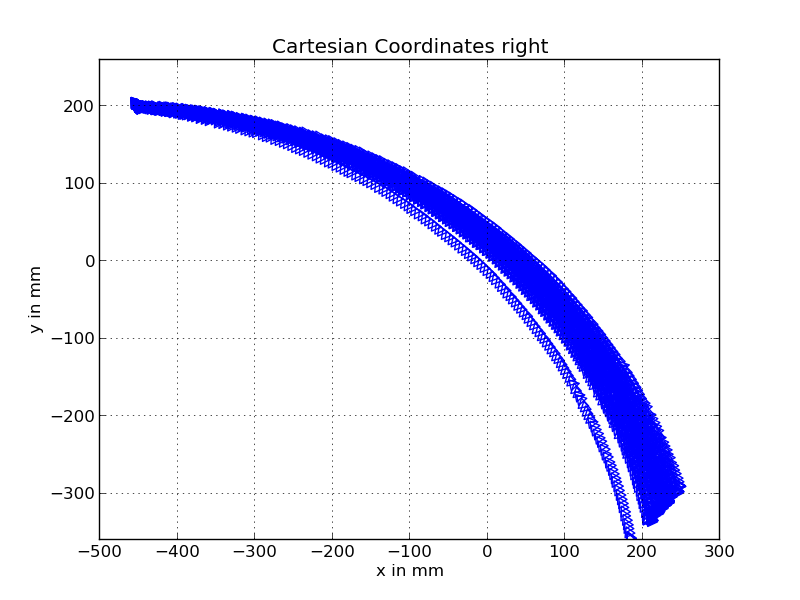
\includegraphics[width=.8\linewidth]{img/right_outliers.png}
  %\caption{}
  %\label{fig:}
\end{minipage}%
\begin{minipage}{.5\textwidth}
  \centering
  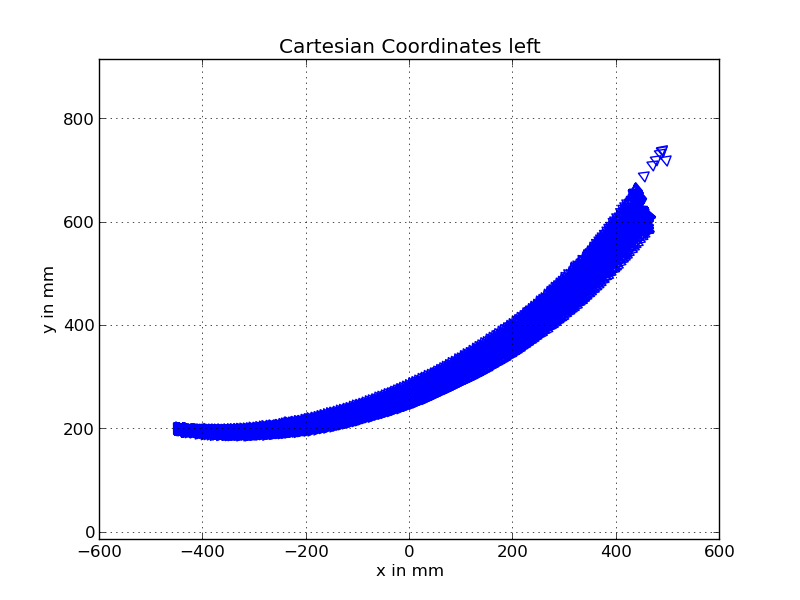
\includegraphics[width=.8\linewidth]{img/left_outlier.png}
  %\caption{}
  %\label{fig:} 
\end{minipage}
\caption{Outliers.}
\label{fig:outliers}
\end{figure}


\section{Recordings}
The pose was recorded in roll, pitch and yaw. We only use roll because the robot can not leave the ground. The roll is depicted as the orientation of the triangle in the Figures below.\\

\subsection{Ahead}
%AHEAD
\begin{figure}[H]
\centering
\begin{minipage}{.5\textwidth}
  \centering
  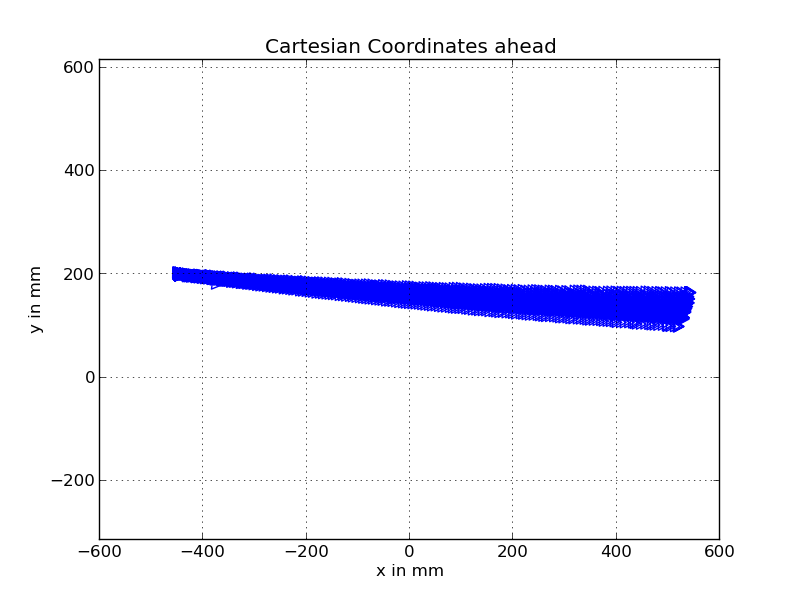
\includegraphics[width=.8\linewidth]{img/ahead_c.png}
  %\caption{}
  %\label{fig:}
\end{minipage}%
\begin{minipage}{.5\textwidth}
  \centering
  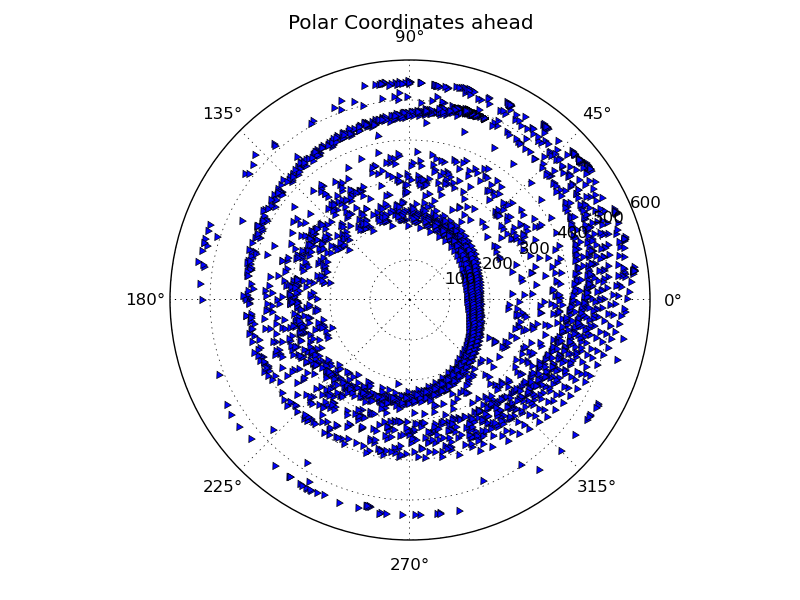
\includegraphics[width=.8\linewidth]{img/ahead_pc_c.png}
  %\caption{}
  %\label{fig:} 
\end{minipage}
\caption{Recordings of the ahead movements in cartesian and polar coordinates.}
\label{fig:ahead}
\end{figure}
%Description
%AHEAD
\begin{figure}[H]
\centering
\begin{minipage}{.5\textwidth}
  \centering
  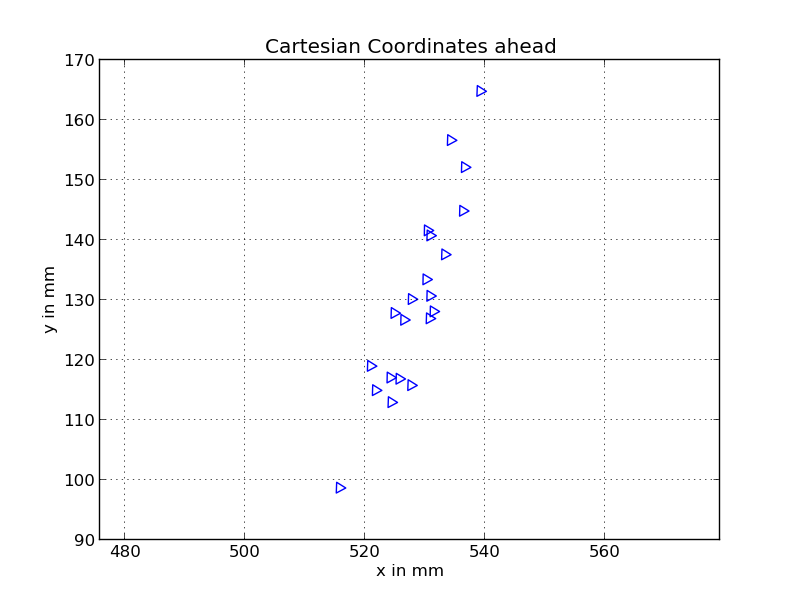
\includegraphics[width=.8\linewidth]{img/ahead_f.png}
  %\caption{}
  %\label{fig:}
\end{minipage}%
\begin{minipage}{.5\textwidth}
  \centering
  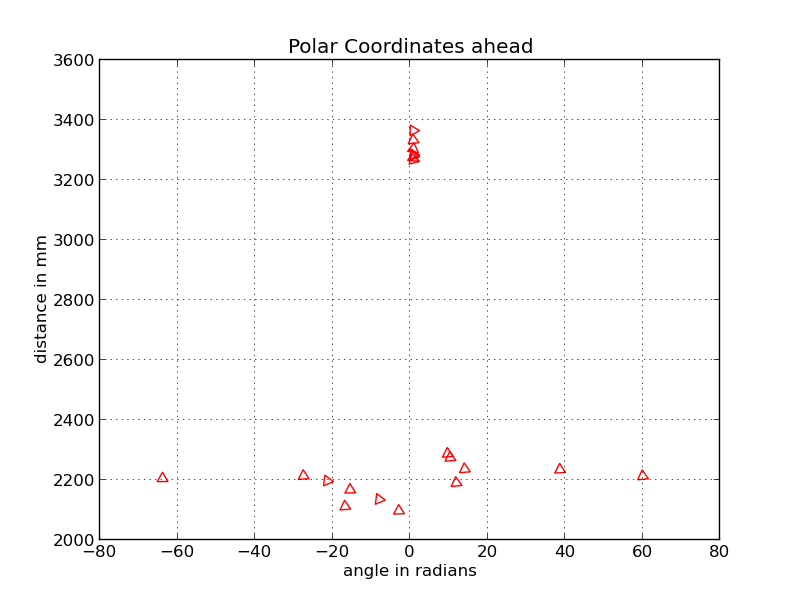
\includegraphics[width=.8\linewidth]{img/ahead_pc_f.png}
  %\caption{}
  %\label{fig:} 
\end{minipage}
\caption{Final positions of the ahead movements in cartesian and polar coordinates.}
\label{fig:ahead_f}
\end{figure}
%Description
%AHEAD
\begin{figure}[H]
\centering
\begin{minipage}{.5\textwidth}
  \centering
  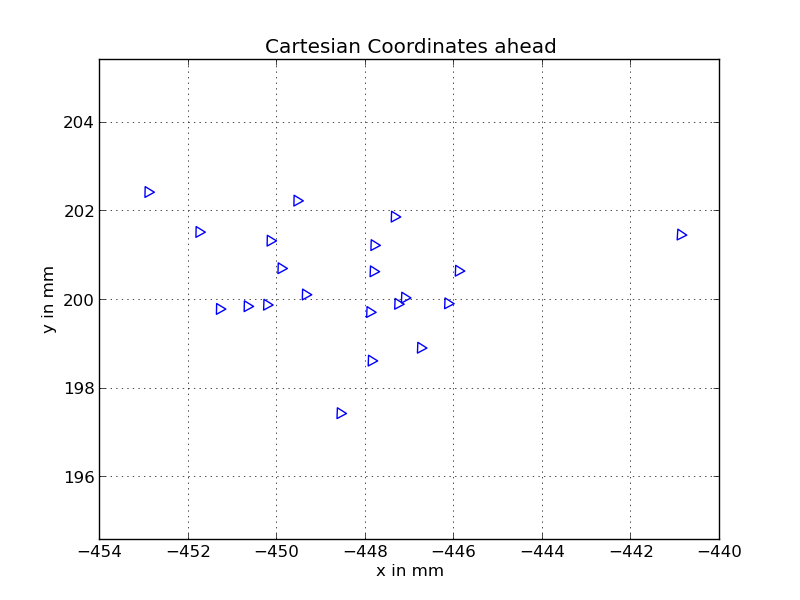
\includegraphics[width=.8\linewidth]{img/ahead_s.png}
  %\caption{}
  %\label{fig:}
\end{minipage}%
\begin{minipage}{.5\textwidth}
  \centering
  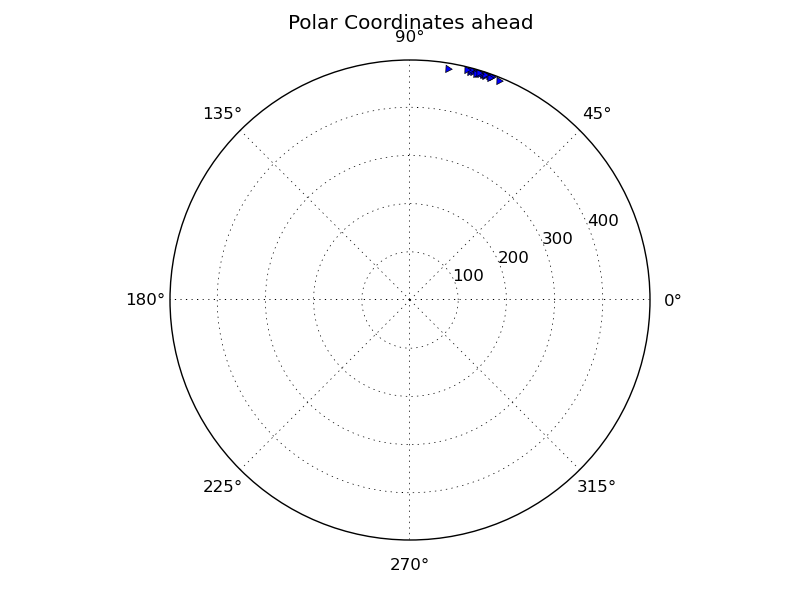
\includegraphics[width=.8\linewidth]{img/ahead_pc_s.png}
  %\caption{}
  %\label{fig:} 
\end{minipage}
\caption{Starting positions of the ahead movements in cartesian and polar coordinates.}
\label{fig:ahead_s}
\end{figure}
%Description


\subsection{Left}
%LEFT
\begin{figure}[H]
\centering
\begin{minipage}{.5\textwidth}
  \centering
  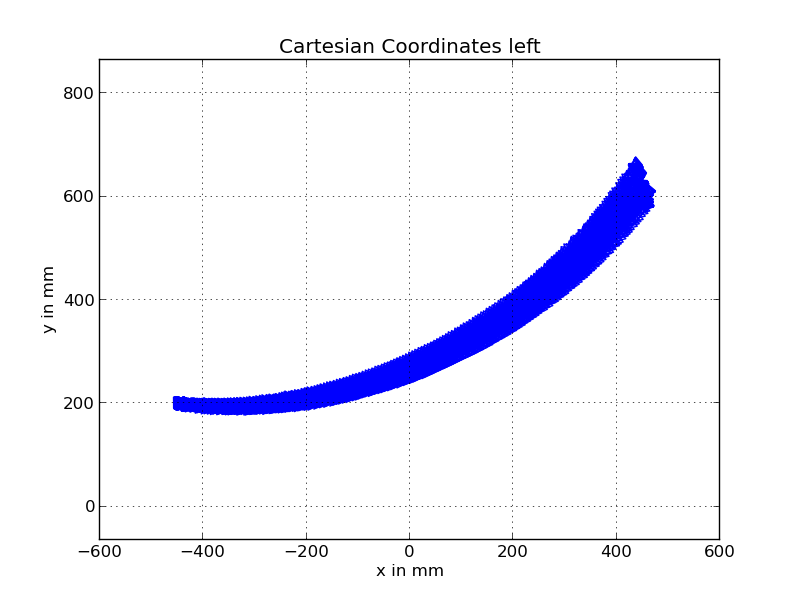
\includegraphics[width=.8\linewidth]{img/left_c.png}
  %\caption{}
  %\label{fig:}
\end{minipage}%
\begin{minipage}{.5\textwidth}
  \centering
  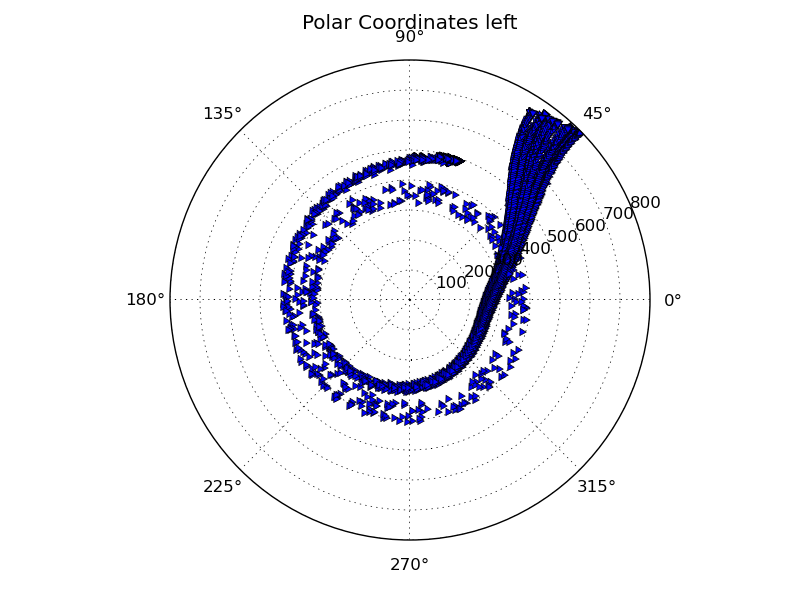
\includegraphics[width=.8\linewidth]{img/left_pc_c.png}
  %\caption{}
  %\label{fig:} 
\end{minipage}
\caption{Recordings of the left movements in cartesian and polar coordinates.}
\label{fig:left}
\end{figure}
%Description

%LEFT
\begin{figure}[H]
\centering
\begin{minipage}{.5\textwidth}
  \centering
  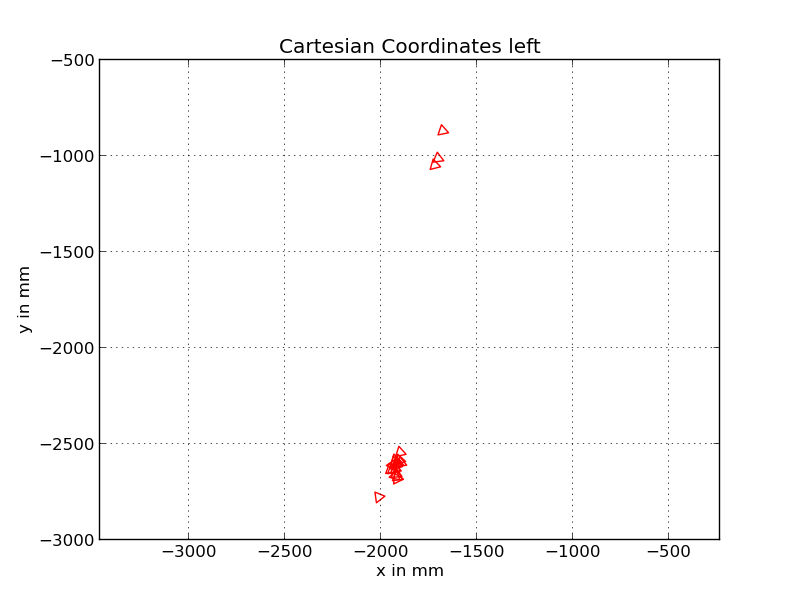
\includegraphics[width=.8\linewidth]{img/left_f.png}
  %\caption{}
  %\label{fig:}
\end{minipage}%
\begin{minipage}{.5\textwidth}
  \centering
  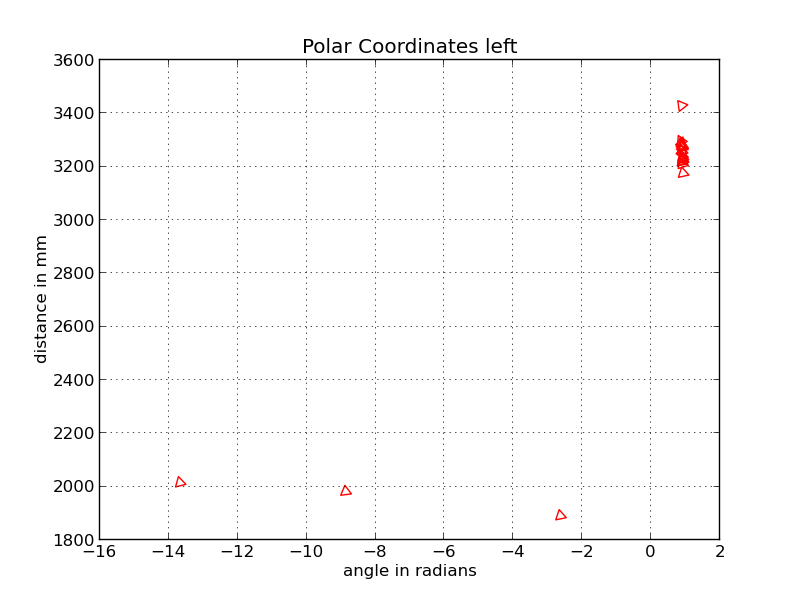
\includegraphics[width=.8\linewidth]{img/left_pc_f.png}
  %\caption{}
  %\label{fig:} 
\end{minipage}
\caption{Final positions of the recordings of the left movements in cartesian and polar coordinates.}
\label{fig:left_f}
\end{figure}
%Description

%LEFT
\begin{figure}[H]
\centering
\begin{minipage}{.5\textwidth}
  \centering
  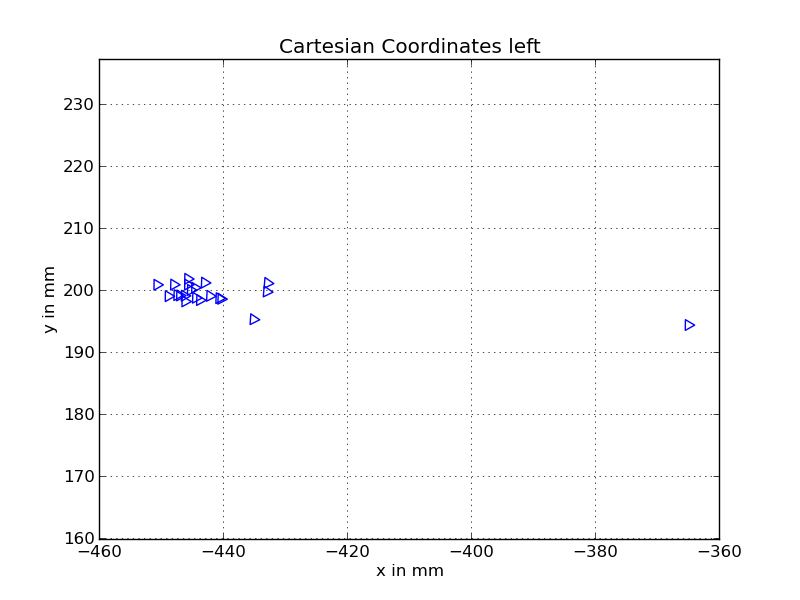
\includegraphics[width=.8\linewidth]{img/left_s.png}
  %\caption{}
  %\label{fig:}
\end{minipage}%
\begin{minipage}{.5\textwidth}
  \centering
  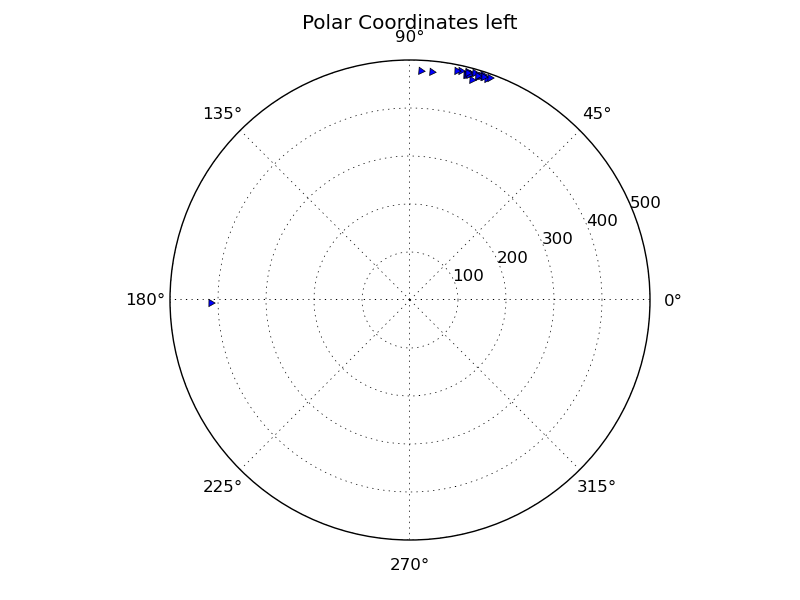
\includegraphics[width=.8\linewidth]{img/left_pc_s.png}
  %\caption{}
  %\label{fig:} 
\end{minipage}
\caption{Starting positions of the recordings of the left movements in cartesian and polar coordinates.}
\label{fig:left_s}
\end{figure}
%Description


\subsection{Right}
%RIGHT
\begin{figure}[H]
\centering
\begin{minipage}{.5\textwidth}
  \centering
  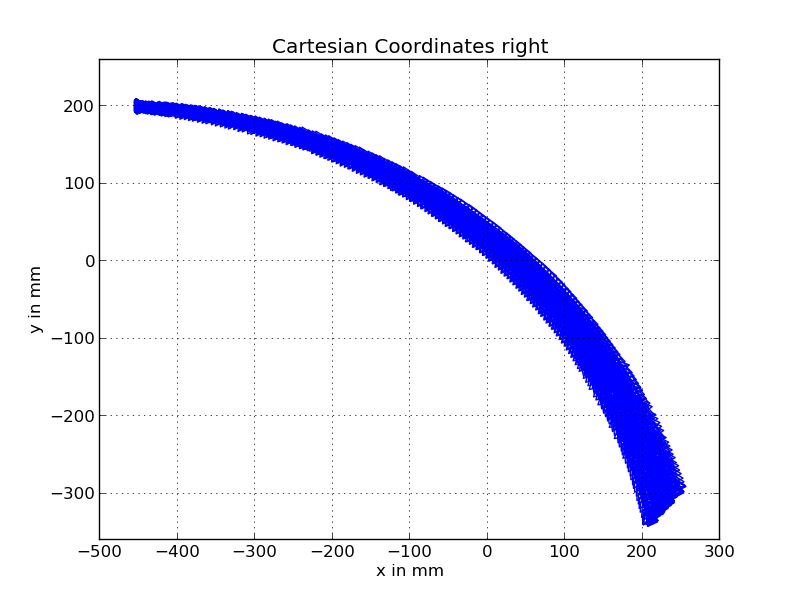
\includegraphics[width=.8\linewidth]{img/right_c.png}
  %\caption{}
  %\label{fig:}
\end{minipage}%
\begin{minipage}{.5\textwidth}
  \centering
  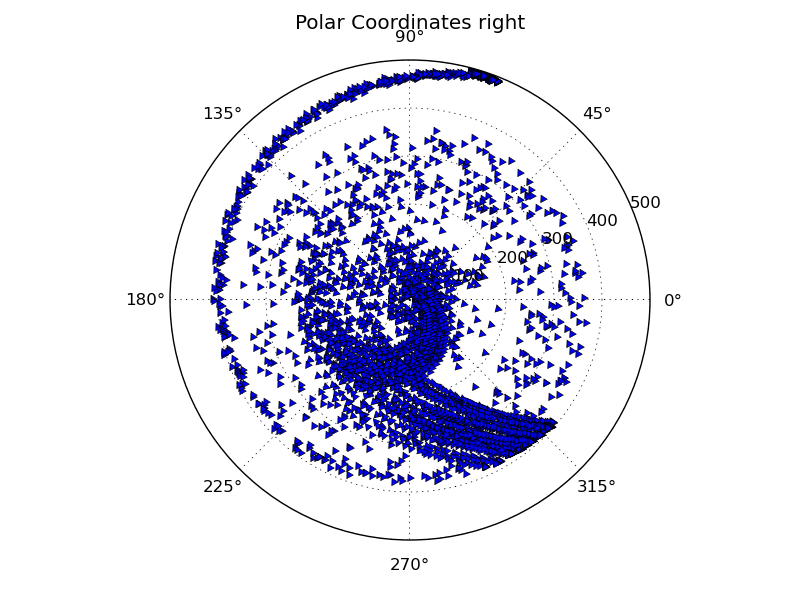
\includegraphics[width=.8\linewidth]{img/right_pc_c.png}
  %\caption{}
  %\label{fig:} 
\end{minipage}
\caption{Recordings of the right movements in cartesian and polar coordinates.}
\label{fig:right}
\end{figure}
%Description

%RIGHT
\begin{figure}[H]
\centering
\begin{minipage}{.5\textwidth}
  \centering
  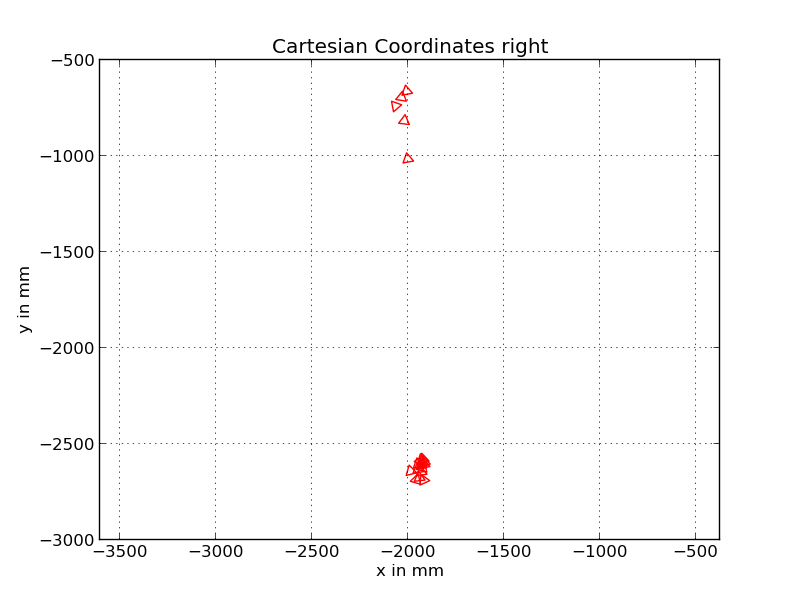
\includegraphics[width=.8\linewidth]{img/right_f.png}
  %\caption{}
  %\label{fig:}
\end{minipage}%
\begin{minipage}{.5\textwidth}
  \centering
  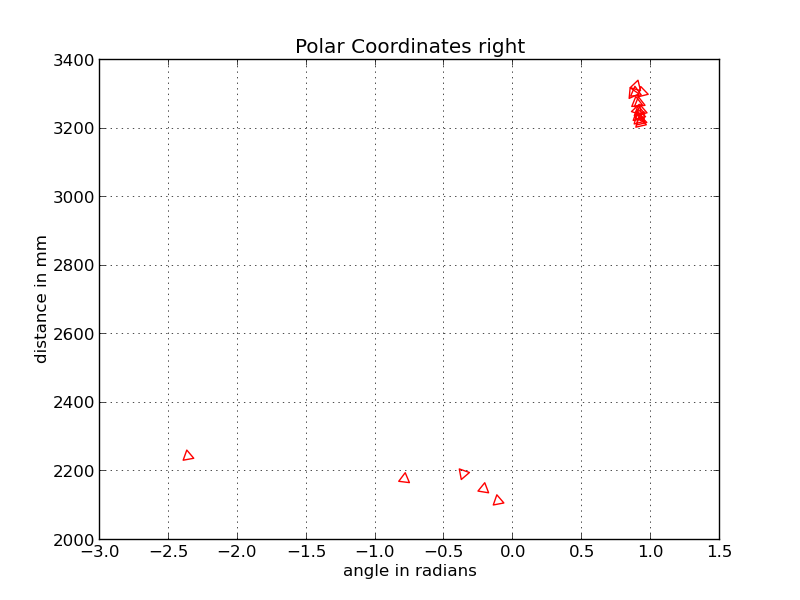
\includegraphics[width=.8\linewidth]{img/right_pc_f.png}
  %\caption{}
  %\label{fig:} 
\end{minipage}
\caption{Final positions of the recordings of the right movements in cartesian and polar coordinates.}
\label{fig:right}
\end{figure}
%Description

%RIGHT
\begin{figure}[H]
\centering
\begin{minipage}{.5\textwidth}
  \centering
  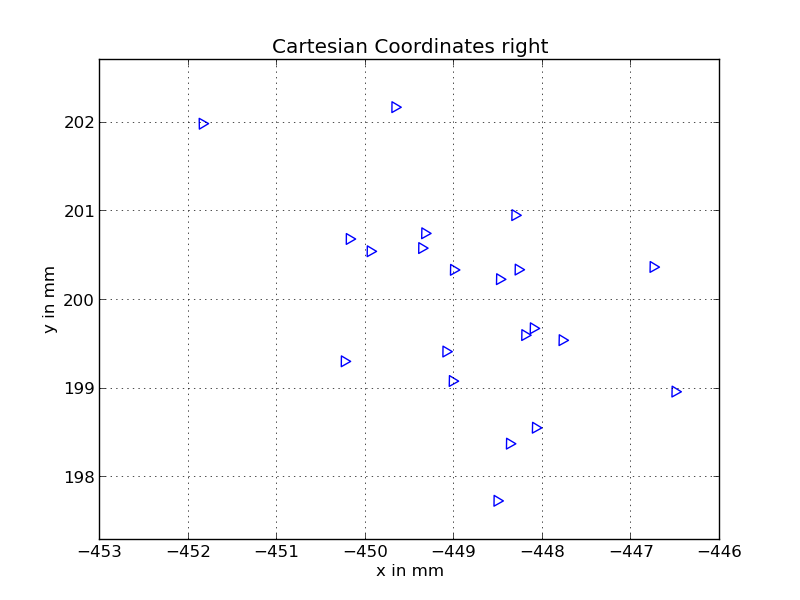
\includegraphics[width=.8\linewidth]{img/right_s.png}
  %\caption{}
  %\label{fig:}
\end{minipage}%
\begin{minipage}{.5\textwidth}
  \centering
  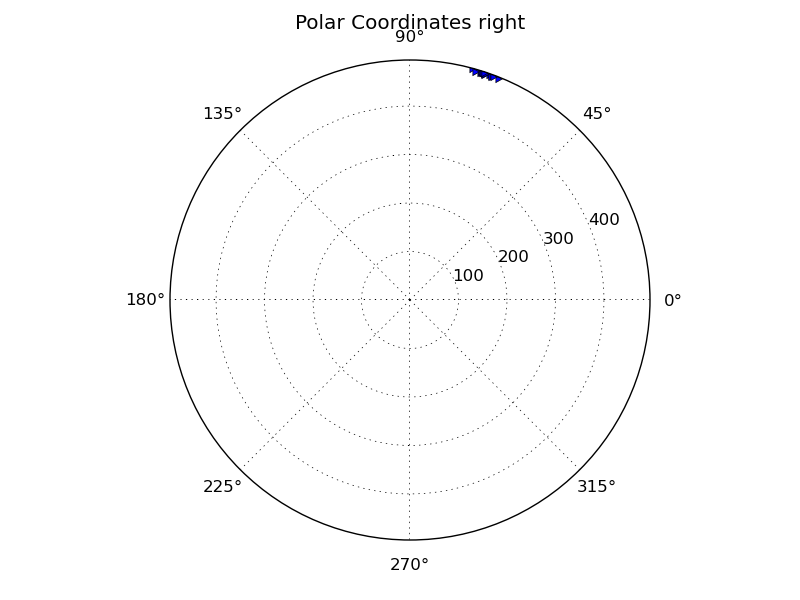
\includegraphics[width=.8\linewidth]{img/right_pc_s.png}
  %\caption{}
  %\label{fig:} 
\end{minipage}
\caption{Starting positions of the recordings of the right movements in cartesian and polar coordinates.}
\label{fig:right}
\end{figure}


\subsection{Box Plots}

\begin{figure}[H]
\centering
\begin{minipage}{.5\textwidth}
  \centering
  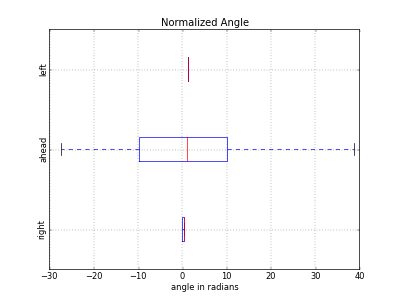
\includegraphics[width=.8\linewidth]{img/BoxplotAngleNorm_f.png}
  %\caption{}
  %\label{fig:}
\end{minipage}%
\begin{minipage}{.5\textwidth}
  \centering
  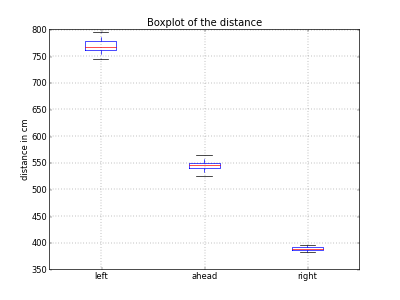
\includegraphics[width=.8\linewidth]{img/BoxplotDistance_f.png}
  %\caption{}
  %\label{fig:} 
\end{minipage}
\caption{Boxplots of the normed angles and the distances of the final positions.}
\label{fig:right}
\end{figure}
%Description


\begin{figure}[H]
\centering
\begin{minipage}{.5\textwidth}
  \centering
  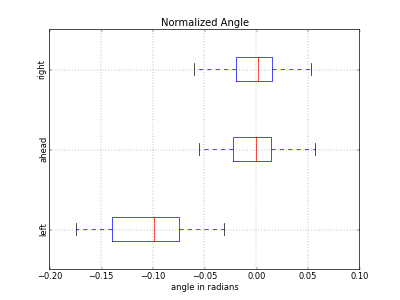
\includegraphics[width=.8\linewidth]{img/BoxplotAngleNorm_s.png}
  %\caption{}
  %\label{fig:}
\end{minipage}%
\begin{minipage}{.5\textwidth}
  \centering
  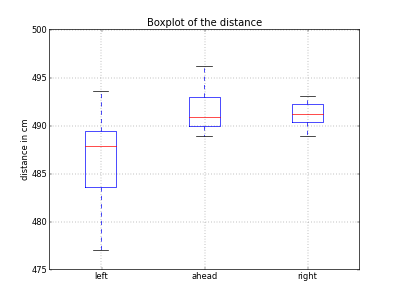
\includegraphics[width=.8\linewidth]{img/BoxplotDistance_s.png}
  %\caption{}
  %\label{fig:} 
\end{minipage}
\caption{Boxplots of the normed angles and the distances of the starting positions.}
\label{fig:right}
\end{figure}
%Description



\subsection{Distributions}
We plotted the histogram of the final positions, determined the normal distributions and made a p-test for their fit. The calculated values can be found in the appendix.

\subsubsection{left}
\begin{figure}[H]
\centering
\begin{minipage}{.5\textwidth}
  \centering
  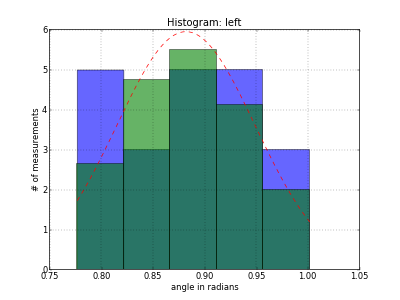
\includegraphics[width=1.0\linewidth]{img/Angles_left_f.png}
  %\caption{}
  %\label{fig:}
\end{minipage}%
\begin{minipage}{.5\textwidth}
  \centering
  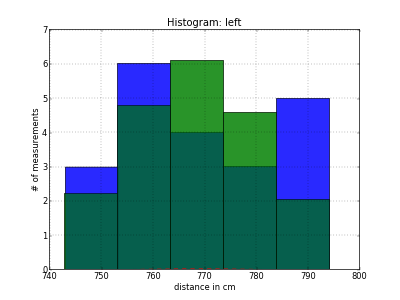
\includegraphics[width=1.0\linewidth]{img/Distances_left_f.png}
  %\caption{}
  %\label{fig:}
\end{minipage}
\caption{Histograms of the angles and distances of the final positions of the left run (blue) and their normal distribution (red, green).}
\end{figure}
%Description

\begin{figure}[H]
\centering
\begin{minipage}{.5\textwidth}
  \centering
  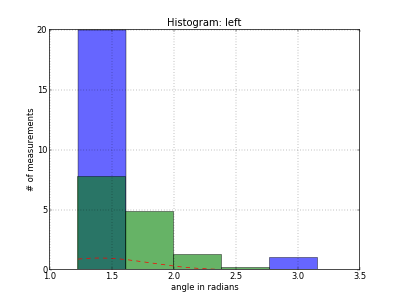
\includegraphics[width=1.0\linewidth]{img/Angles_left_s.png}
  %\caption{}
  %\label{fig:}
\end{minipage}%
\begin{minipage}{.5\textwidth}
  \centering
  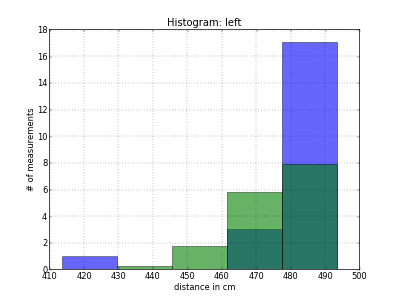
\includegraphics[width=1.0\linewidth]{img/Distances_left_s.png}
  %\caption{}
  %\label{fig:}
\end{minipage}
\caption{Histograms of the angles and distances of the starting positions of the left run (blue) and their normal distribution (red, green).}
\end{figure}
%Description


\subsubsection{ahead}
\begin{figure}[H]
\centering
\begin{minipage}{.5\textwidth}
  \centering
  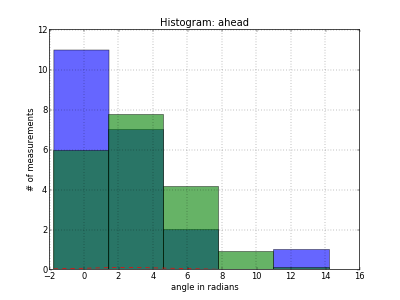
\includegraphics[width=1.0\linewidth]{img/Angles_ahead_f.png}
  %\caption{}
  %\label{fig:}
\end{minipage}%
\begin{minipage}{.5\textwidth}
  \centering
  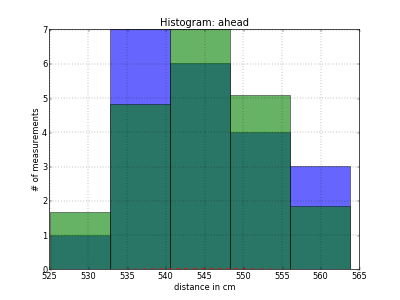
\includegraphics[width=1.0\linewidth]{img/Distances_ahead_f.png}
  %\caption{}
  %\label{fig:}
\end{minipage}
\caption{Histograms of the angles and distances of the final positions of the run straight ahead(blue) and their normal distribution (red, green).}
\end{figure}
%Description

\begin{figure}[H]
\centering
\begin{minipage}{.5\textwidth}
  \centering
  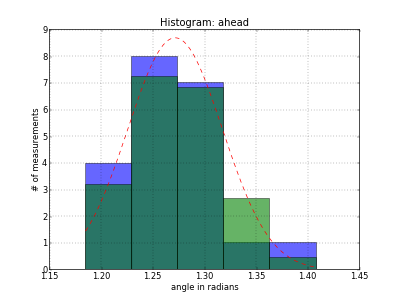
\includegraphics[width=1.0\linewidth]{img/Angles_ahead_s.png}
  %\caption{}
  %\label{fig:}
\end{minipage}%
\begin{minipage}{.5\textwidth}
  \centering
  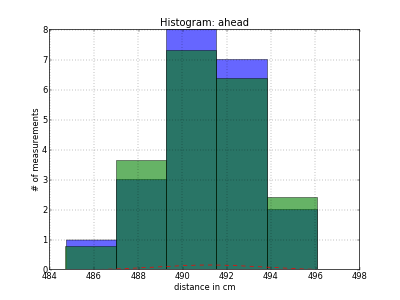
\includegraphics[width=1.0\linewidth]{img/Distances_ahead_s.png}
  %\caption{}
  %\label{fig:}
\end{minipage}
\caption{Histograms of the angles and distances of the starting positions of the run straight ahead(blue) and their normal distribution (red, green).}
\end{figure}
%Description

\subsubsection{right}

\begin{figure}[H]
\centering
\begin{minipage}{.5\textwidth}
  \centering
  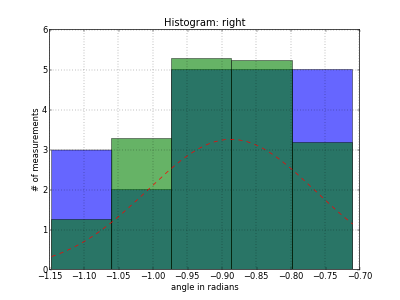
\includegraphics[width=1.0\linewidth]{img/Angles_right_f.png}
  %\caption{}
  %\label{fig:}
\end{minipage}%
\begin{minipage}{.5\textwidth}
  \centering
  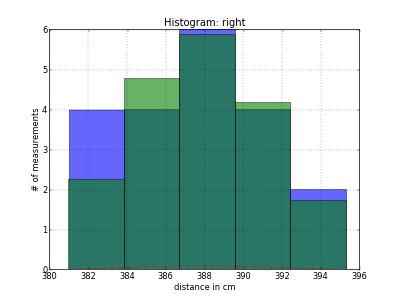
\includegraphics[width=1.0\linewidth]{img/Distances_right_f.png}
  %\caption{}
  %\label{fig:}
\end{minipage}
\caption{Histograms of the angles and distances of  the final positions of the right run(blue) and their normal distribution (red, green).}
\end{figure}

\begin{figure}[H]
\centering
\begin{minipage}{.5\textwidth}
  \centering
  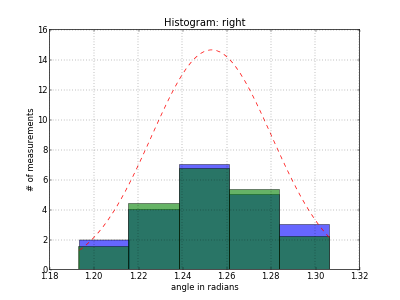
\includegraphics[width=1.0\linewidth]{img/Angles_right_s.png}
  %\caption{}
  %\label{fig:}
\end{minipage}%
\begin{minipage}{.5\textwidth}
  \centering
  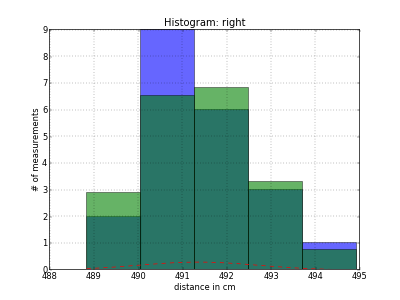
\includegraphics[width=1.0\linewidth]{img/Distances_right_s.png}
  %\caption{}
  %\label{fig:}
\end{minipage}
\caption{Histograms of the angles and distances of  the starting positions of the right run(blue) and their normal distribution (red, green).}
\end{figure}


%\section{Conclusions}
%TODO: CONCLUSIONS



\section{Appendix}
\subsection{Histograms of the final positions}
See histogram\_f.out
\lstinputlisting[language=python]{histogram_f.out}

\subsection{Histograms of the starting positions}
See histogram\_s.out
\lstinputlisting[language=python]{histogram_s.out}

\subsection{Code}
See final\_graphics.py\\
For a complete view see \href{https://github.com/ChrisQuignon/SEE/tree/master/Homework04}{github.com/ChrisQuignon/SEE}
\lstinputlisting[language=python]{graphics.py}



%BIBLIOGRPAHY!
\bibliographystyle{plain}%amsalpha
\bibliography{bib.bib}
%\bibentry{}


%COPY AND PASTE FROM HERE

%\begin{enumerate}
% \item
%\end{enumerate}

%\href{link}{text}

%\begin[Language=Python]{lstlisting}
%#PYTHON CODE HERE
%\end{lstlisting}

%\lstinputlisting[language=Java]{ }

%\csvautotabular[separator=semicolon]{data.csv}

%\begin{figure}
% \center
% \includegraphics[width= cm]{img/ }
% \caption{}
%\end{figure}



\end{document}
